\documentclass[tikz,border=12pt]{standalone}
\usepackage[utf8]{inputenc}
\usepackage{tikz}
\usetikzlibrary{shapes,arrows.meta,positioning,calc}

\definecolor{ScoutGreen}{HTML}{005432}
\definecolor{ScoutNavy}{HTML}{002855}
\definecolor{ScoutBlue}{HTML}{006EB6}
\definecolor{ScoutRed}{HTML}{A31920}
\definecolor{ScoutAmber}{HTML}{D97706}
\definecolor{BorderGray}{HTML}{CBD5E1}

\begin{document}
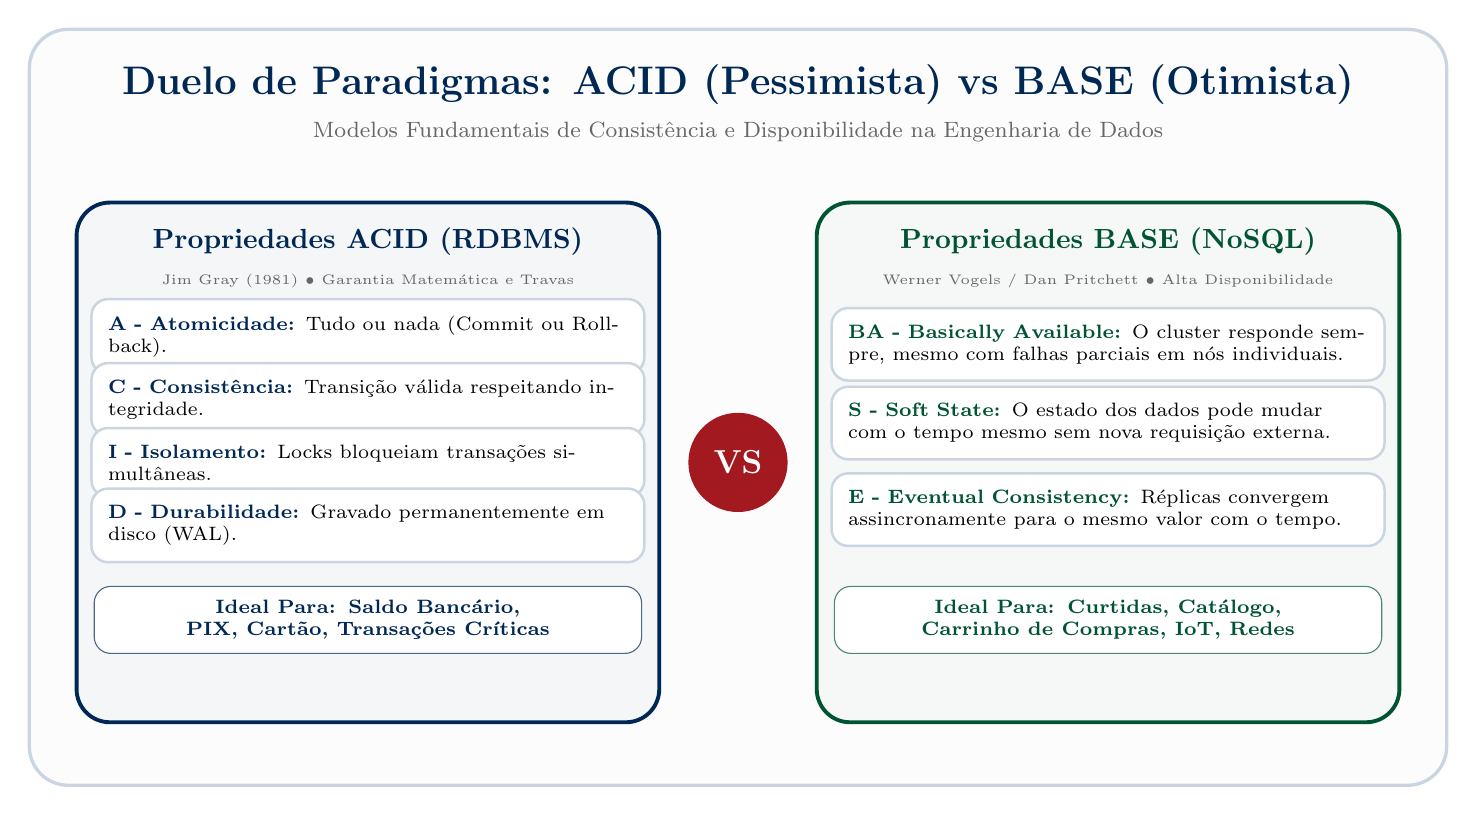
\begin{tikzpicture}[
    font=\sffamily,
    card/.style={draw=#1, rounded corners=12pt, fill=#1!4, line width=1.4pt, inner sep=8pt},
    itembox/.style={draw=BorderGray, rounded corners=6pt, fill=white, line width=0.9pt, align=left, inner sep=6pt}
]

  % Painel Fundo Geral
  \node[draw=BorderGray, rounded corners=14pt, fill=gray!2, line width=1.2pt, minimum width=18.0cm, minimum height=9.6cm] (bg) at (0, 0) {};
  
  \node[font=\bfseries\Large, text=ScoutNavy] at (0, 4.1) {Duelo de Paradigmas: ACID (Pessimista) vs BASE (Otimista)};
  \node[font=\footnotesize, text=gray!80!black] at (0, 3.5) {Modelos Fundamentais de Consistência e Disponibilidade na Engenharia de Dados};

  % =========================================================================
  % CARD ESQUERDO: ACID
  % =========================================================================
  \node[card=ScoutNavy, minimum width=7.4cm, minimum height=6.6cm] (c_acid) at (-4.7, -0.7) {};
  
  \node[font=\bfseries\normalsize, text=ScoutNavy] at (-4.7, 2.1) {Propriedades ACID (RDBMS)};
  \node[font=\tiny, text=gray!80!black] at (-4.7, 1.6) {Jim Gray (1981) $\bullet$ Garantia Matemática e Travas};

  \node[itembox, text width=6.6cm, font=\scriptsize] at (-4.7, 0.9) {
    \textbf{\color{ScoutNavy}A - Atomicidade:} Tudo ou nada (Commit ou Rollback).
  };
  \node[itembox, text width=6.6cm, font=\scriptsize] at (-4.7, 0.1) {
    \textbf{\color{ScoutNavy}C - Consistência:} Transição válida respeitando integridade.
  };
  \node[itembox, text width=6.6cm, font=\scriptsize] at (-4.7, -0.7) {
    \textbf{\color{ScoutNavy}I - Isolamento:} Locks bloqueiam transações simultâneas.
  };
  \node[itembox, text width=6.6cm, font=\scriptsize] at (-4.7, -1.5) {
    \textbf{\color{ScoutNavy}D - Durabilidade:} Gravado permanentemente em disco (WAL).
  };

  \node[draw=ScoutNavy!70, fill=white, rounded corners=6pt, font=\scriptsize\bfseries, text=ScoutNavy, align=center, text width=6.6cm, inner sep=5pt] at (-4.7, -2.7) {
    Ideal Para: Saldo Bancário, PIX, Cartão, Transações Críticas
  };

  % =========================================================================
  % VS CENTRAL (ESPAÇO LIVRE DE 2.0 CM)
  % =========================================================================
  \node[circle, fill=ScoutRed, text=white, font=\bfseries\large, inner sep=6pt] at (0, -0.7) {VS};

  % =========================================================================
  % CARD DIREITO: BASE
  % =========================================================================
  \node[card=ScoutGreen, minimum width=7.4cm, minimum height=6.6cm] (c_base) at (4.7, -0.7) {};
  
  \node[font=\bfseries\normalsize, text=ScoutGreen] at (4.7, 2.1) {Propriedades BASE (NoSQL)};
  \node[font=\tiny, text=gray!80!black] at (4.7, 1.6) {Werner Vogels / Dan Pritchett $\bullet$ Alta Disponibilidade};

  \node[itembox, text width=6.6cm, font=\scriptsize] at (4.7, 0.8) {
    \textbf{\color{ScoutGreen}BA - Basically Available:} O cluster responde sempre, mesmo com falhas parciais em nós individuais.
  };
  \node[itembox, text width=6.6cm, font=\scriptsize] at (4.7, -0.2) {
    \textbf{\color{ScoutGreen}S - Soft State:} O estado dos dados pode mudar com o tempo mesmo sem nova requisição externa.
  };
  \node[itembox, text width=6.6cm, font=\scriptsize] at (4.7, -1.3) {
    \textbf{\color{ScoutGreen}E - Eventual Consistency:} Réplicas convergem assincronamente para o mesmo valor com o tempo.
  };

  \node[draw=ScoutGreen!70, fill=white, rounded corners=6pt, font=\scriptsize\bfseries, text=ScoutGreen, align=center, text width=6.6cm, inner sep=5pt] at (4.7, -2.7) {
    Ideal Para: Curtidas, Catálogo, Carrinho de Compras, IoT, Redes
  };

\end{tikzpicture}
\end{document}
